\chapter{Eredmények}
\pagestyle{headings}

Dolgozatom fő eredménye a pásztázó referencia elektród technikához szükséges mikroméretű másodfajú elektródok megtervezése és elkészítése, illetve a kiértékelési módszerek lépésről lépésre történő bemutatása. Az elektródok és a módszer helyes működésének bemutatására megjósolható viselkedésű rendszereket tanulmányoztam; egy polarizált grafit elektródpárt és egy vas-cink galvánpárt. Munkám eredménye tehát elsősorban nem a méréseim eredménye -- hiszen az egyszerű vas-cink galvánpár korróziója már régóta jól ismert -- hanem annak összehasonlítása a vártakkal.

\section{Grafit modellcéltárgy}
\subsection{Potenciáltérképezések}
%Mint korábban említettem már, a pásztázó elektrokémiai mikroszkópiában általában egy céltárgy felszínét vizsgáljuk vagy az azon lejátszódó folyamatról szeretnénk információhoz jutni. 

Először egy jól ismert modellrendszert vizsgáltam meg; az előzőekben részletesebben jellemzett grafit elektródpárt. A céltárgy két elektródját 2000 mV-al polarizáltam egymáshoz képest a méréshez is használt, \emph{Módszerek} fejezetben említett eDAQ mérőműszer egyik csatornáját potenciosztátként használva. A pásztázási terület horizontális esetben 4000x3000 $\upmu$m$^2$ volt az X-Y síkon, Z irányban 200 $\upmu$m eltolással a két mérés között. Vertikális pásztázás esetén 5000x1000 $\upmu$m$^2$ volt az X-Z síkon a vizsgált terület. A feltérképezett katód környezetében hidrogén-ion redukciójára, az anódos oldalon pedig oxigéngáz fejlődésre számíthatunk, a következő egyenletek szerint:

\begin{equation}
2\textrm{H}^+ + 2e^- \longrightarrow \textrm{H}_2
\label{grafit_katod}
\end{equation}

\begin{equation}
2\textrm{OH}^- \longrightarrow 0.5 \textrm{O}_2 + \textrm{H}_2\textrm{O} + 2e^-
\label{grafit_anod}
\end{equation}

\begin{figure}
\centering
\includegraphics[width=0.3\textwidth, angle=-90]{img/mérések/Fe_h_100.eps}\includegraphics[width=0.3\textwidth, angle=-90]{img/mérések/Fe_h_500.eps}

\includegraphics[width=0.3\textwidth, angle=-90]{img/mérések/Zn_h_100.eps}\includegraphics[width=0.3\textwidth, angle=-90]{img/mérések/Zn_h_500.eps}

\includegraphics[width=0.3\textwidth, angle=-90]{img/mérések/grafit_h1_100.eps}
\includegraphics[width=0.3\textwidth, angle=-90]{img/mérések/grafit_h_300.eps}
\caption{A céltárgyakról készült horizontális potenciáltérképek:
(AB) a vas katód 100 $\upmu$m és 500 $\upmu$m magasságban, (CD) a cink anód 100 $\upmu$m és 500 $\upmu$m magasságban és (EF) a grafit katódja és anódja 100 $\upmu$m és 300 $\upmu$m magasságban mérve}
\label{fig:horizontális}
\end{figure}

\begin{figure}
\centering
\includegraphics[width=0.3\textwidth, angle=-90]{img/mérések/Fe_v.eps}
\includegraphics[width=0.3\textwidth, angle=-90]{img/mérések/Zn_v.eps}
\includegraphics[width=0.3\textwidth, angle=-90]{img/mérések/grafit_v.eps}
\caption{A céltárgyakról készült vertikális potenciáltérképek:
(A) a vas katód, (B) a cink anód és (C) a grafit katódja és anódja}
\label{fig:vertikális}
\end{figure}

A mikroméretű referenciaelektróddal készített pásztázások horizontális potenciáltérképeit a \ref{fig:horizontális}.EF ábrán, a vertikálisat pedig az \ref{fig:vertikális}C. ábrán láthatjuk. Megközelítőleg 5 mV eltéréssel, nagyjából azonos potenciáltartományba esnek a mérések eredményei, tehát a rendszer a két mérés között nem változott jelentősen. Továbbá jól látható, hogy az elektródpár tagjai a polarizáció hatására katódként (-295 mV körüli átlagérték) és anódként (-265 mV körüli átlagérték) viselkedtek, ahogy arra számítottunk. Így az eredményekből látható, hogy a tanulmányozott rendszer ténylegesen állandó, jól jellemezhető és ez a módszer alkalmazható a potenciáltérképezésre. A modellcéltárgy vizsgálatával tehát megbizonyosodtam róla, hogy a mérőrendszer működőképes.

\subsection{Elektromos mező és az áramsűrűség}
A \emph{Módszerek} című fejezetben említettek szerint elvégeztem a numerikus deriválást és ez alapján ábrázoltam vektorosan az elektromos mezőt (\ref{fig:field_h}C,  \ref{fig:field_h1}C, és \ref{fig:field_v}C. ábrák). Az \ref{fig:field_h}.C ábra és a \ref{fig:field_h1}.C ábra a horizontális pásztázások eredményei, az \ref{fig:field_v}C. ábra pedig a vertikálisé. A Z tengelyen nézve az anód esetében az áramvektorok az oxidáció következtében a síkból kifelé mutatnak a kationok mozgási irányának megfelelően, a katódnál a redukció miatt pedig a síkba mutatnak. Az X-Y sík ábrán pedig az anódból a katód felé irányulnak a vetorok. A szakirodalomban megtalálható, SVET technikát alkalmazó mérésekhez nagyon hasonló eredményeket kaptam \cite{bastos2016preliminary}. 

Az előző fejezetben leírtak alapján elkészítettem az áramsűrűség Z irányú komponensének térképét a horizontális pásztázásra. Jól látható az \ref{fig:áramsűrűség}C. ábrán, hogy a piros színnel jelölt katód helyén és környezetében negatív értékeket kaptam, a kék színnel jelölt anód esetében pedig pozitív értékeket, ahogy vártuk. Az ábra zölddel jelölt részén körülbelül 0-nak tekinthető az áramerősség. Továbbá megfigyelhetjük, hogy körülbelül szimmetrikusnak mondható a katód és anód régiójában az áramerősség, ami távolódva a középpontjuktól csökkenést mutat. Ez a térkép az elektromos mezőével mutat hasonlóságot, mivel az előzőleg már említett \ref{eq:nabla}. egyenlet szerint a két érték között egyenes arányosság van \cite{isaacs1981scanning,bastos2017application}.

\section{Vas-cink galvánpár korrózió vizsgálata}
\subsection{Potenciáltérképezések}
Az előző alfejezetben bemutatott grafit céltárgy vizsgálatával megbizonyosodtam az általam készített elektródok és a kiértékelési módszerem helyességéről, hiszen a várttal egyező eredményeket kaptam az egyszerű grafit modellrendszerre. Ezután nekiláttam a vas-cink galvánpárból készült céltárgy tanulmányozásának, melyet a \emph{Módszerek} fejezetben jellemeztem részletesebben. A pásztázási terület az anód és katód esetében is 3000x2000 $\upmu$m$^2$ volt az X-Y síkon, horizontális mérések esetén és két horizontális mérés között 400 $\upmu$m Z irányú eltolást alkalmaztam. Vertikális mérések során ez 3000x1000 $\upmu$m$^2$ volt az X-Z síkon. Ez egy gyakori galvanikus rendszer, mivel a vas ötvözeteit, illetve magát a vasat is, számos esetben vonjuk be a jobb korrózióállóság miatt cinkréteggel. Ezt a technikát a hétköznapi életben horganyzásnak hívjuk, amivel jelentős mértékben csökkenthető a védett fém korróziója. Ez annak tulajdonítható, hogy a cink tölti be az \emph{Irodalom} fejezetben említett áldozati anód szerepét a galvanikus kapcsolat során. Tehát a cink oxidálódik a védett fém, vagyis a vas helyett. Ezzel egyidőben a vason redukció zajlik, viszont vaskioldódás nélkül. A cella szétkapcsolása esetén, lokális anód és katód alakulna ki a vas felületén. Elvesztené a cink anódos védelmét és elindulna a rozsdásodás folyamata.
A védett vason végbemenő folyamatnak is a lényege a hidrogén-ion redukció, ahogy az előző alfejezetben jellemzett grafit katód esetén is (\ref{grafit_katod} egyenlet). A cink anódon viszont az előzőektől eltérően maga az elektród oxidálódik:


\begin{equation}
\textrm{Zn} \longrightarrow \textrm{Zn}^{2+} + 2e^- 
\label{cink_anod}
\end{equation}


A vizsgálatok potenciáltérképei az \ref{fig:horizontális}. és \ref{fig:vertikális}. ábrákon láthatóak. Ebben az esetben külön pásztáztam a katód (\ref{fig:horizontális}. ábra AB) és az anód (\ref{fig:horizontális}. ábra CD) felületét, mivel a cink és vas elektródok egymástól túl távol helyezkedtek el. A méréseken jól látszik, hogy felület homogén, vagyis a vas egész felülete katódként viselkedett a cellában a mérés alatt. Ezzel egyeidejűleg a cinkelektród teljes felülete anódként viselkedett. Anódra jellemzően nagyobb (-230 mV körüli) értéket, katód esetében kisebb (-275 mV körüli) értéket mértem. Leolvasható, hogy a potenciáltartomány értékei a pásztázásoknak körülbelül azonos minimum és maximum értéket követnek itt is. A vas vertikális potenciáltérképén (\ref{fig:vertikális}. ábra A) egy szélesebb potenciáltartományt láthatunk, mint a horizontális képén. Ez valószínűleg annak tulajdonítható, hogy a grafittól eltérően, ez a korróziós rendszer időben változó. A vertikális és a horizontális mérések között eltelt idő során a reakció haladt előre, így kaptam kissé eltérő értékeket a két mérésre. 

\subsection{Elektromos mező és az áramsűrűség}

Az előző fejezetben leírtak szerint ábrázoltam vektorosan ebben az esetben is az elektromos mezőt. Az \ref{fig:field_h}.A és \ref{fig:field_h1}.A ábra a vas katód, az \ref{fig:field_h}.B és \ref{fig:field_h1}.B ábra a cink anód horizontális pásztázásainak eredményei, míg az \ref{fig:field_v}.A ábra a vas katód, az \ref{fig:field_v}.B ábra pedig a cink anód vertikális eredményeit mutatják. A Z tengely szerint nézve a vas katód esetében az áramvektorok a síkba befelé mutatnak, az előző alfejezetben leírtak szerint végbemenő redukció miatt (\ref{grafit_katod}. egyenlet). A cink anódnál pedig az említett \ref{cink_anod}. egyenlet szerint lejátszódó oxidáció során képződött ionok miatt a síkból kifelé mutatnak a vektorok.

\begin{figure}
\centering
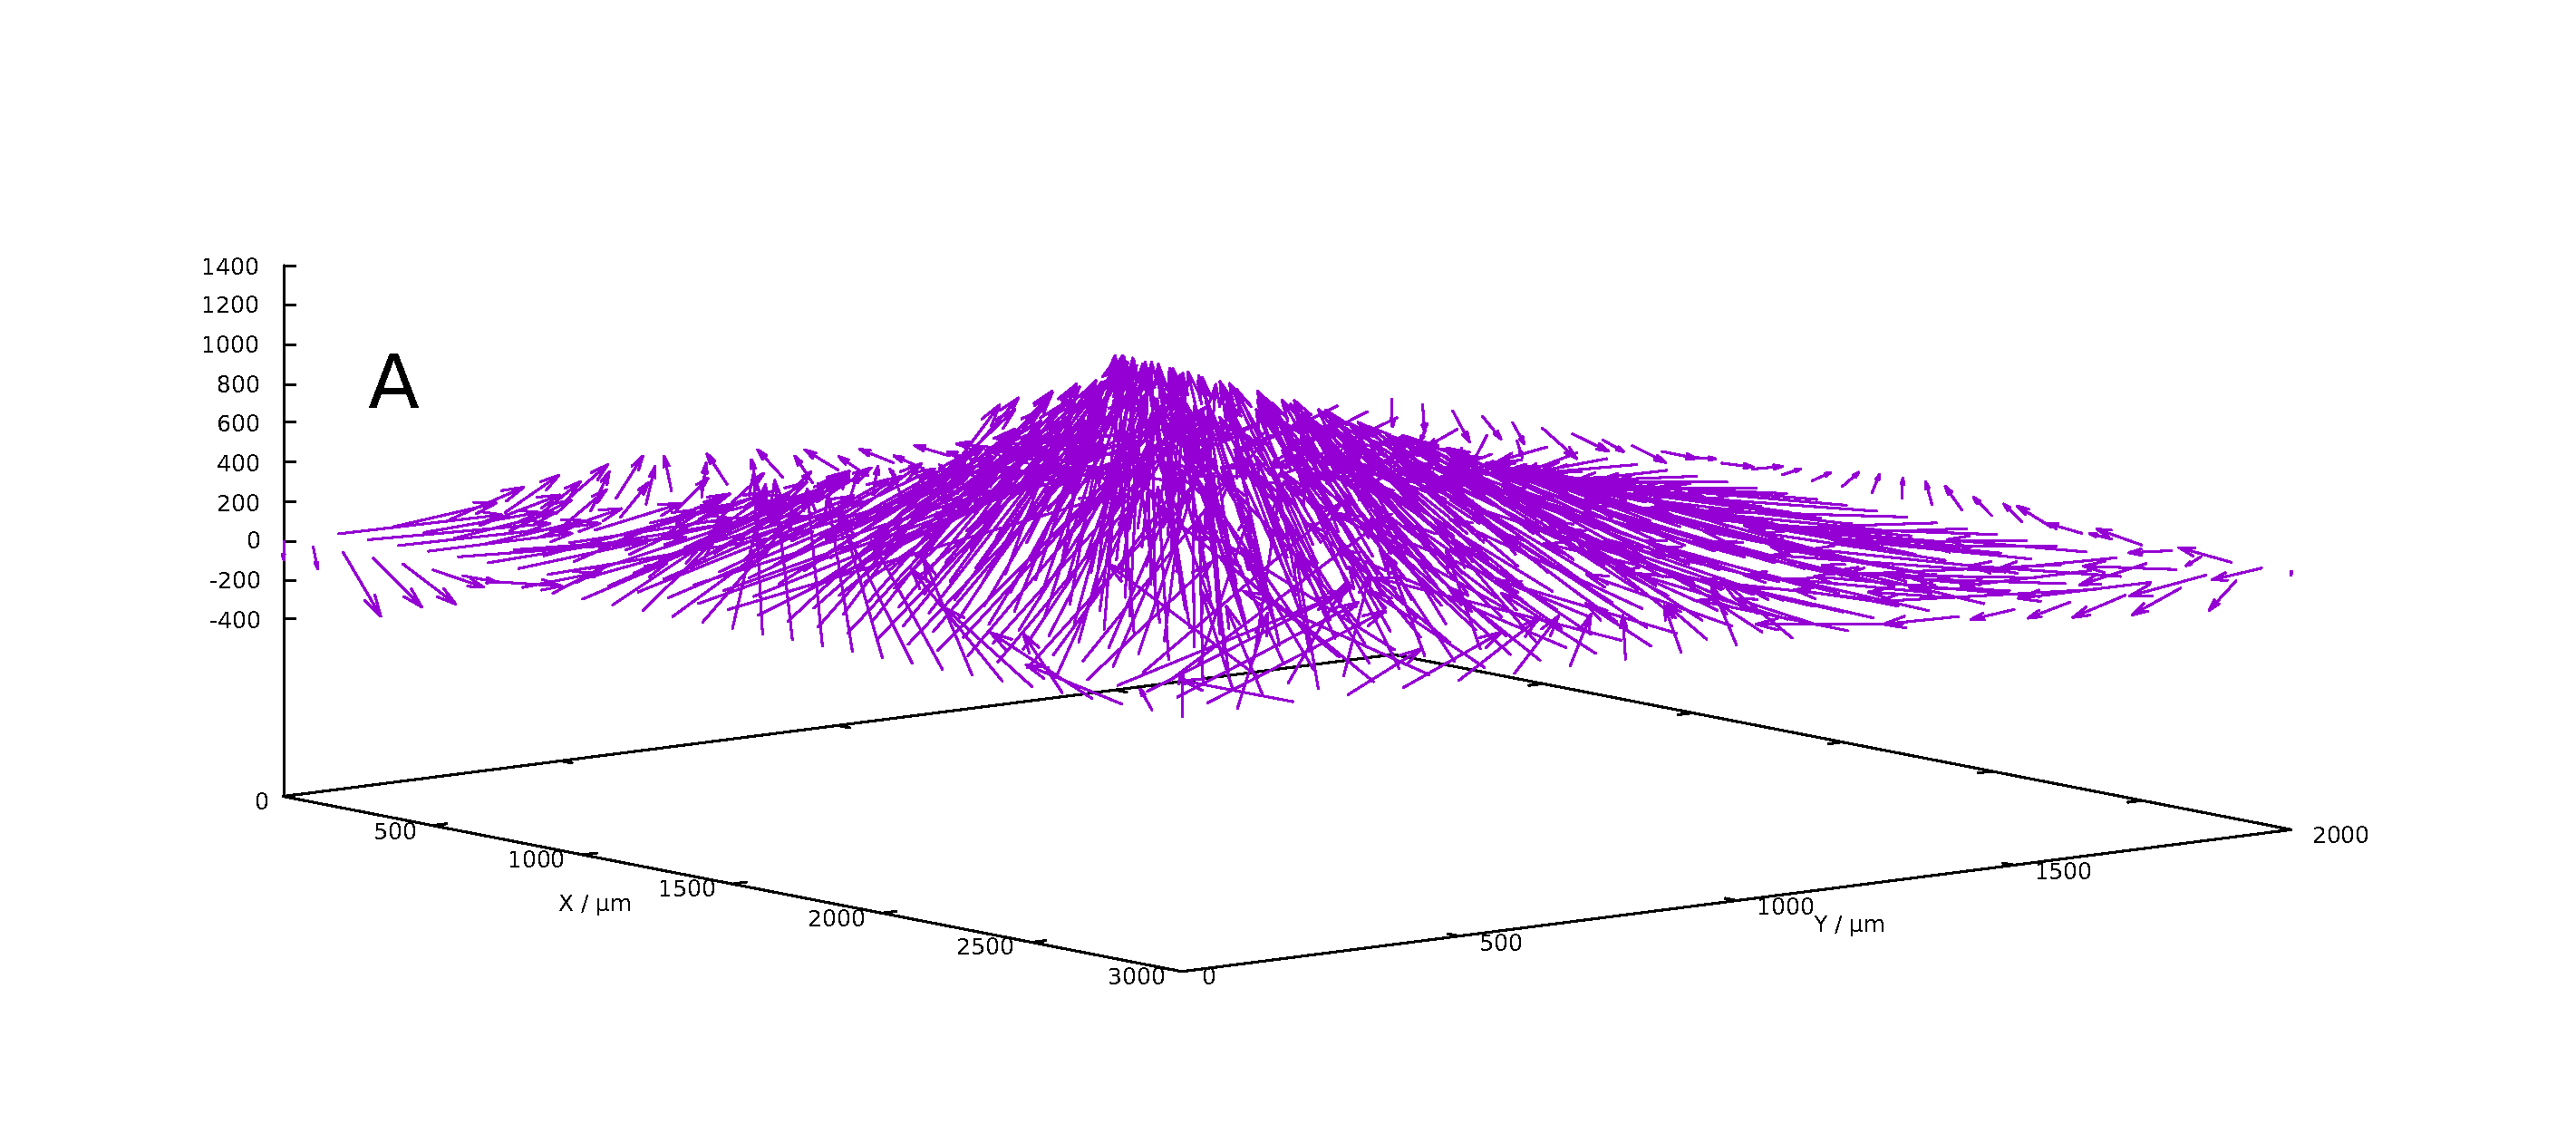
\includegraphics[width=1.2\textwidth]{img/mérések/Fe_h100.pdf}
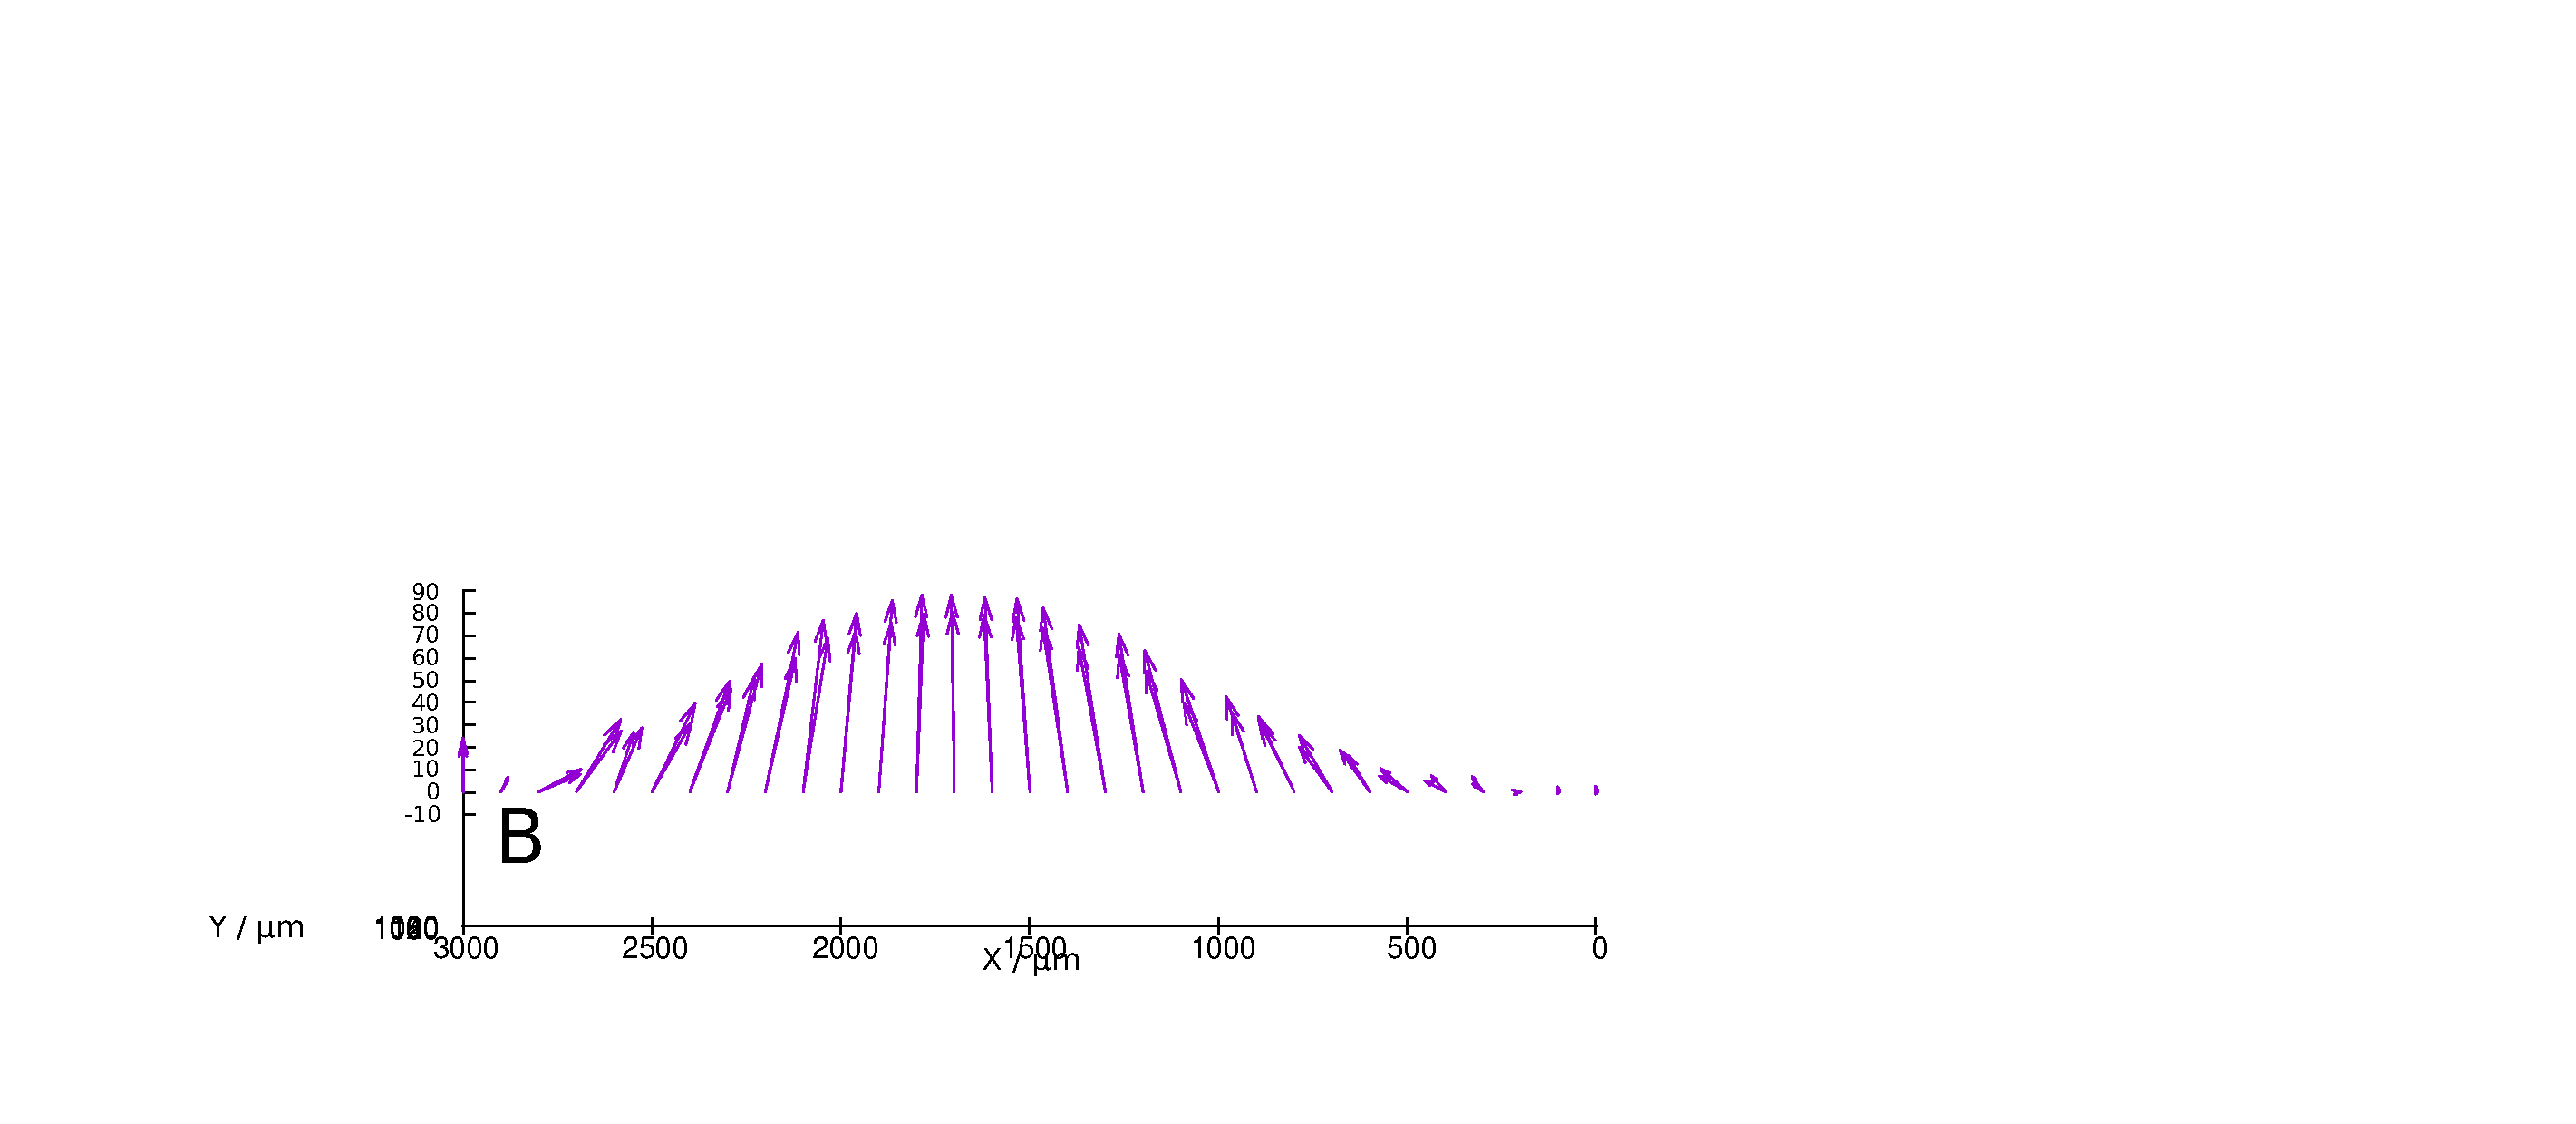
\includegraphics[width=1.2\textwidth]{img/mérések/Zn_h100.pdf}
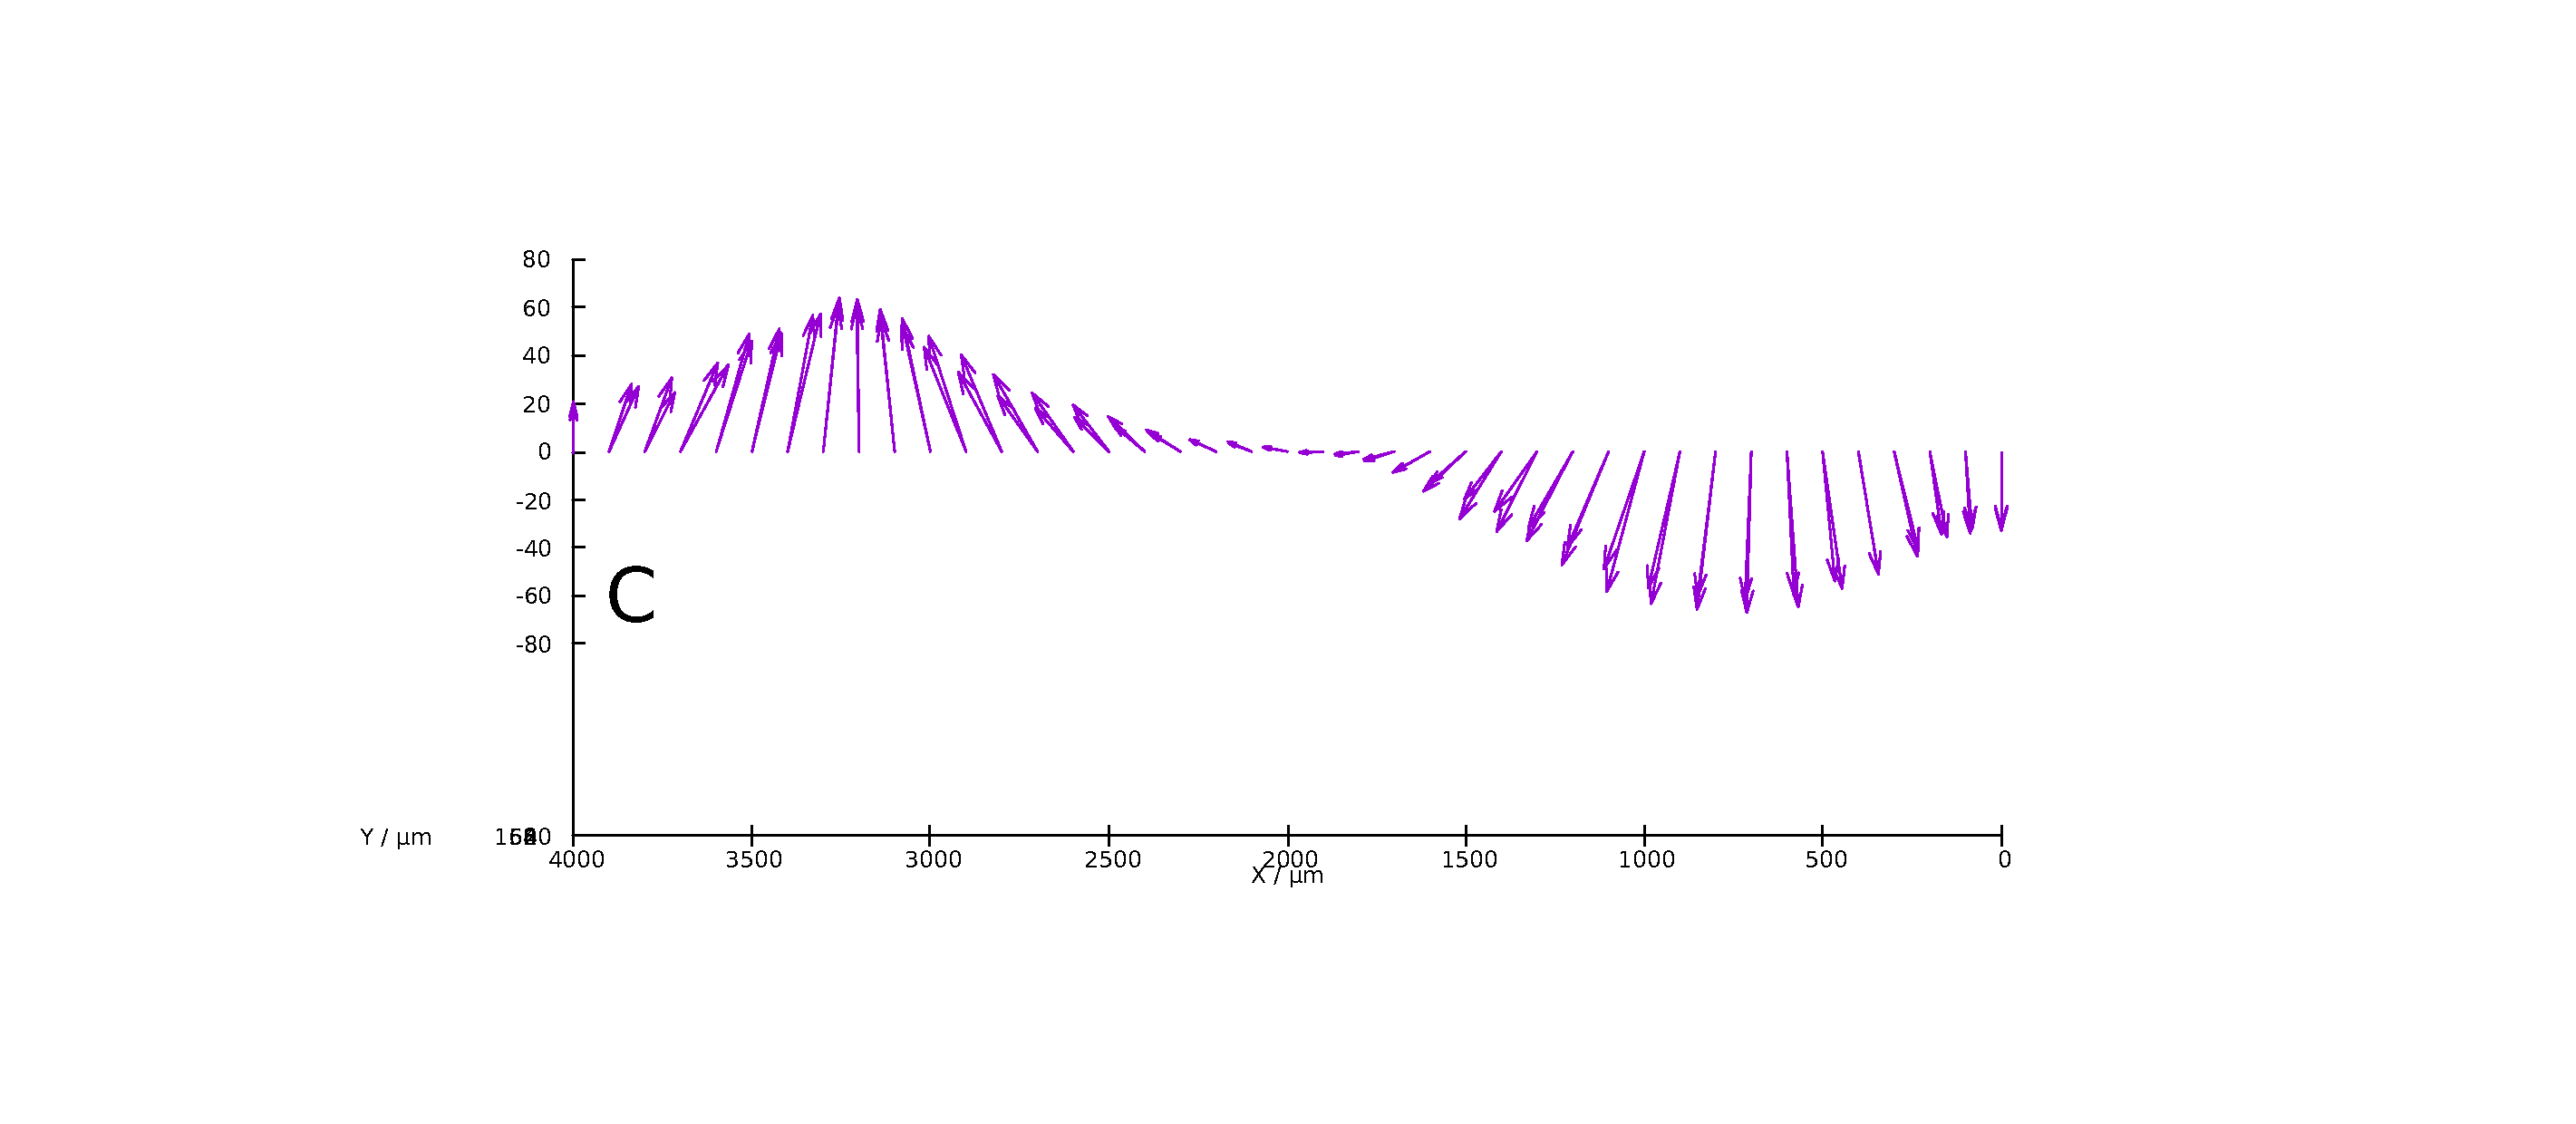
\includegraphics[width=1.2\textwidth]{img/mérések/grafit_h100.pdf}

\caption{Az említett céltárgyakról készült horizontális elektromos mező térképek:
(A) a vas katód, (B) a cink anód és (C) a grafit katódja és anódja 100 $\upmu$m magasságban mérve}
\label{fig:field_h}
\end{figure}


Hasonlóan jártam el a galvánpár esetében is, mikor elkészítettem a horizontális pásztázások áramsűrűség térképét a Z irányú komponens szerint. A grafithoz hasonlóan az anódos áramsűrűség pozitív értéket, a katódos pedig negatív értéket ad. Megfigyelhető az \ref{fig:áramsűrűség}.A ábrán, hogy a vas katód lokális környezetében negatív értékeket kaptam. Ugyanezen ábra (B) képén a cink anód esetében pedig pozitív értékeket, ahogy vártuk. Ezen céltárgynál is elmondhatjuk, hogy körülbelül szimmetrikus a katód és anód régiójában az áramerősség és ez a középpontoktól távolódva csökkenést mutat. A térkép itt is hasonlóságot mutat az elektromos mezőével a korábban említett egyenes arányosság miatt. 

%\includegraphics[trim = 10mm 40mm 0mm 40mm, clip, width=0.4\textwidth, angle=-90]{img/mg_metal/liquid_uncoupled.eps} \includegraphics[trim = 10mm 40mm 0mm 40mm, clip, width=0.4\textwidth, angle=-90]{img/mg_metal/solid_uncoupled.eps}

\begin{figure}
\centering
\includegraphics[width=0.5\textwidth, angle=-90]{img/mérések/Fe1_h100.eps}
\includegraphics[width=0.5\textwidth, angle=-90]{img/mérések/Zn1_h100.eps}
\includegraphics[width=0.5\textwidth, angle=-90]{img/mérések/grafit1_h100.eps}

\caption{A céltárgyakról készült 2D elektromos mező térképek:
(A) a vas katód, (B) a cink anód és (C) a grafit katódja és anódja 100 $\upmu$m magasságban mérve}
\label{fig:field_h1}
\end{figure}

\begin{figure}
\centering
\includegraphics[width=0.35\textwidth, angle=-90]{img/mérések/Fe1_v.eps}
\includegraphics[width=0.35\textwidth, angle=-90]{img/mérések/Zn1_v.eps}
\includegraphics[width=0.35\textwidth, angle=-90]{img/mérések/grafit1_v.eps}

\caption{A céltárgyakról készült vertikális elektromos mező térképek:
(A) a vas katód, (B) a cink anód és (C) a grafit katódja és anódja}
\label{fig:field_v}
\end{figure}

\begin{figure}
\centering
\includegraphics[width=0.5\textwidth, angle=-90]{img/mérések/Fe_h100.eps}
\includegraphics[width=0.5\textwidth, angle=-90]{img/mérések/Zn_h100.eps}
\includegraphics[width=0.5\textwidth, angle=-90]{img/mérések/grafit_h_100.eps}

\caption{A céltárgyakról készült áramsűrűség térképek:
(A) a vas katód, (B) a cink anód és (C) a grafit katódja és anódja}
\label{fig:áramsűrűség}
\end{figure}
